\section{Stabilität}
    \subsection{Stabilitätsprobleme}
        Stetiger oder plötzlicher Übergang zu stabilen aber meistens unerwünschten deformierten Zuständen.\vspace{-1mm}
        \begin{itemize}
            \item Bei welcher Last findet der Übergang statt?
            \item Wie sieht das Deformationsbild aus?
        \end{itemize}
        \begin{center}
            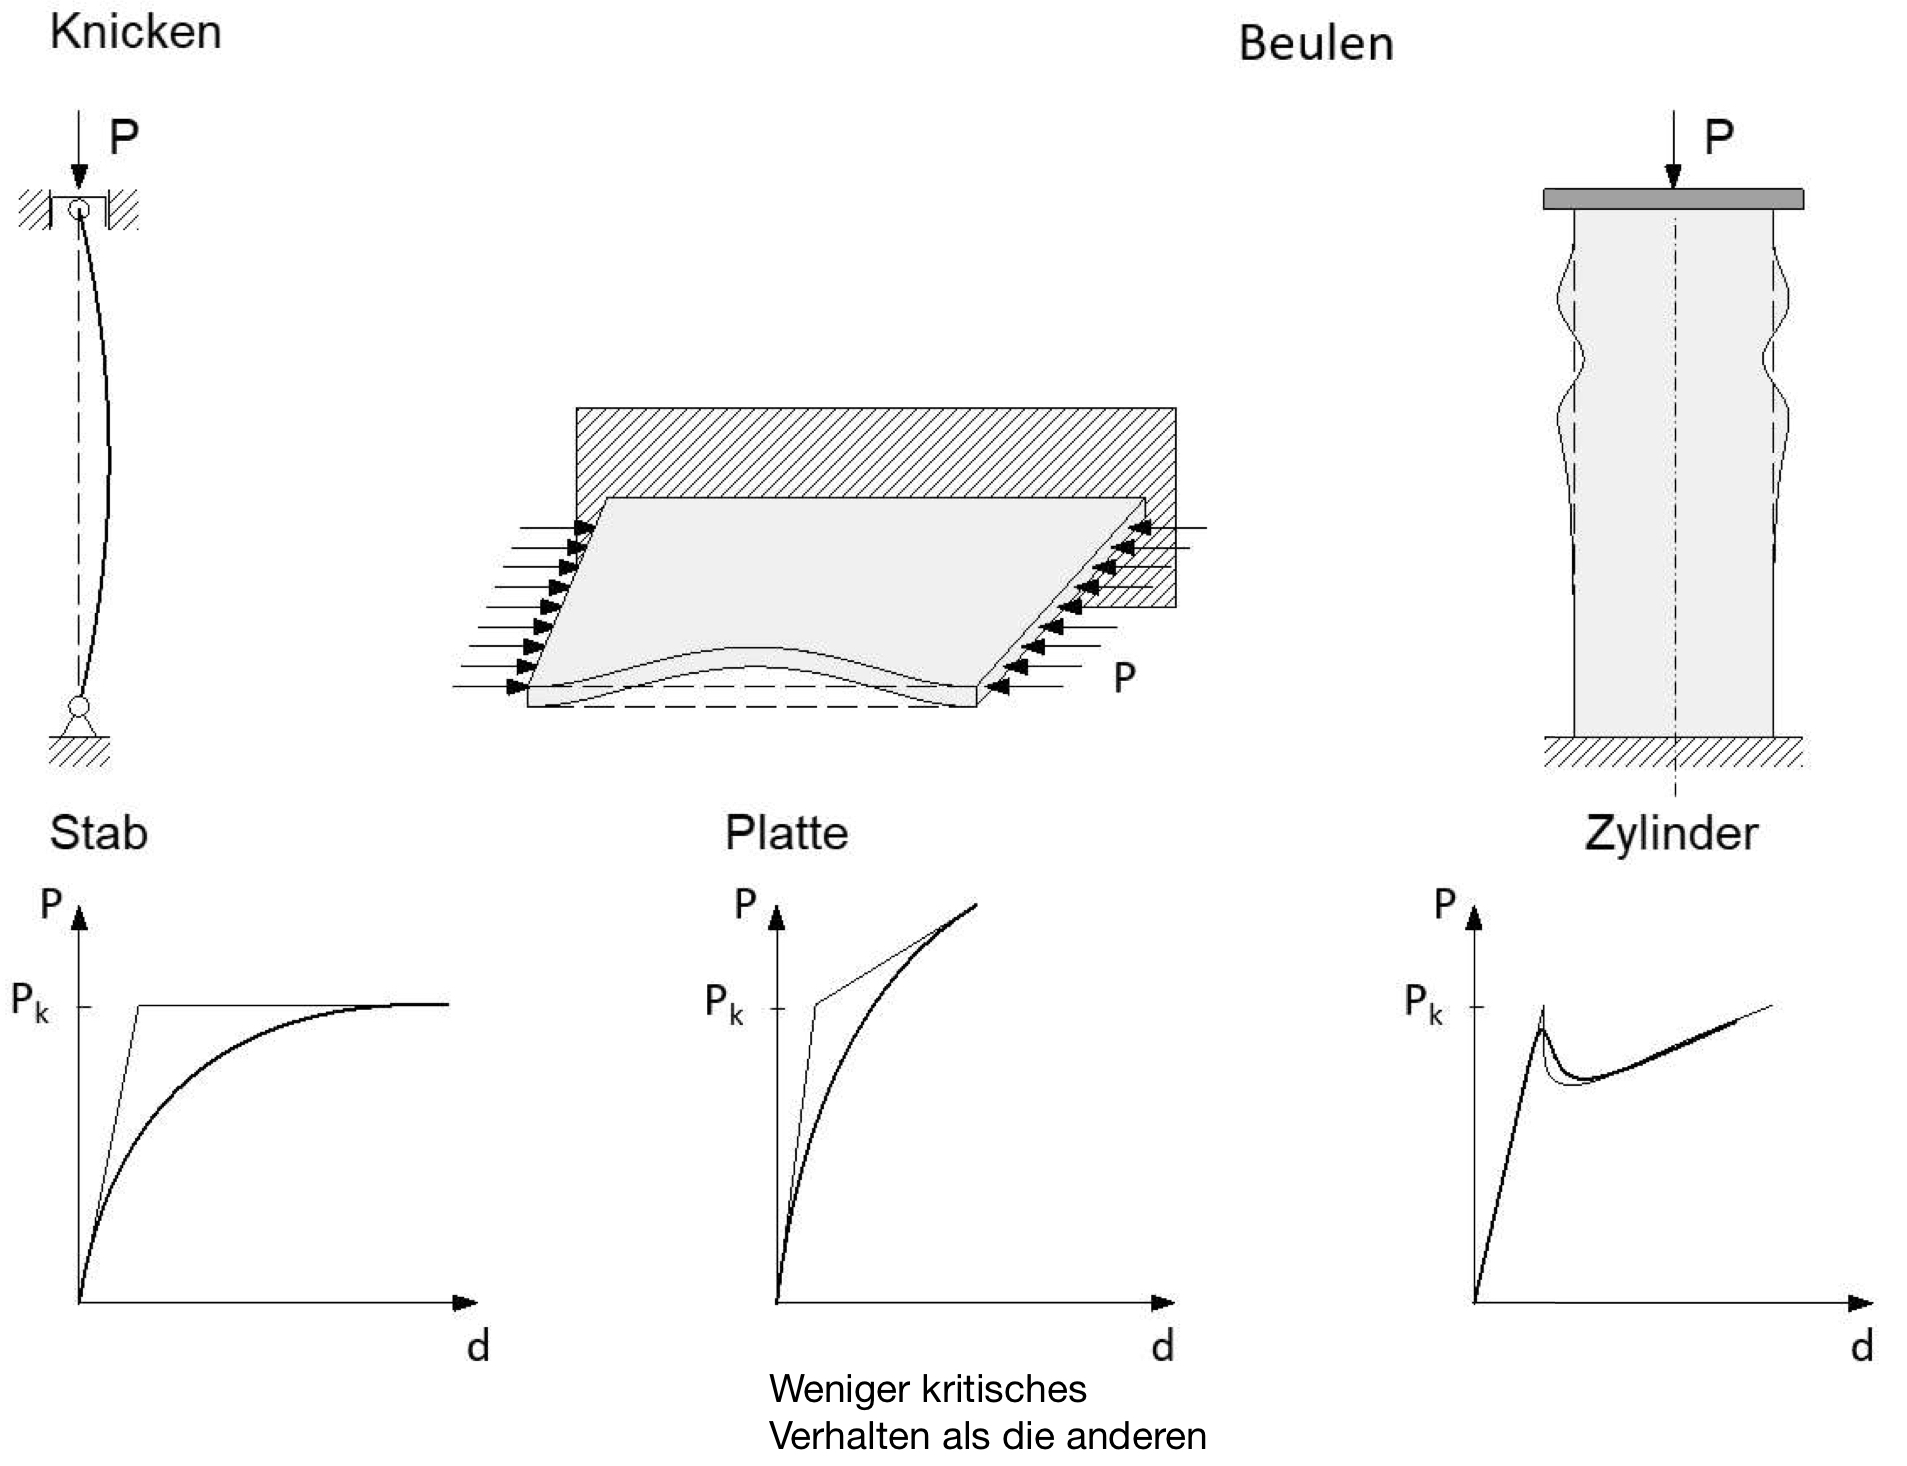
\includegraphics[width=0.7\linewidth, height= 45mm]{09/stability.jpeg}
        \end{center}
    \subsection{1D-Stabilitätsproblem}
        Balken axial belastet, an den Enden axial geführt (oben) und gelenkig gelagert (unten).
        \begin{center}
            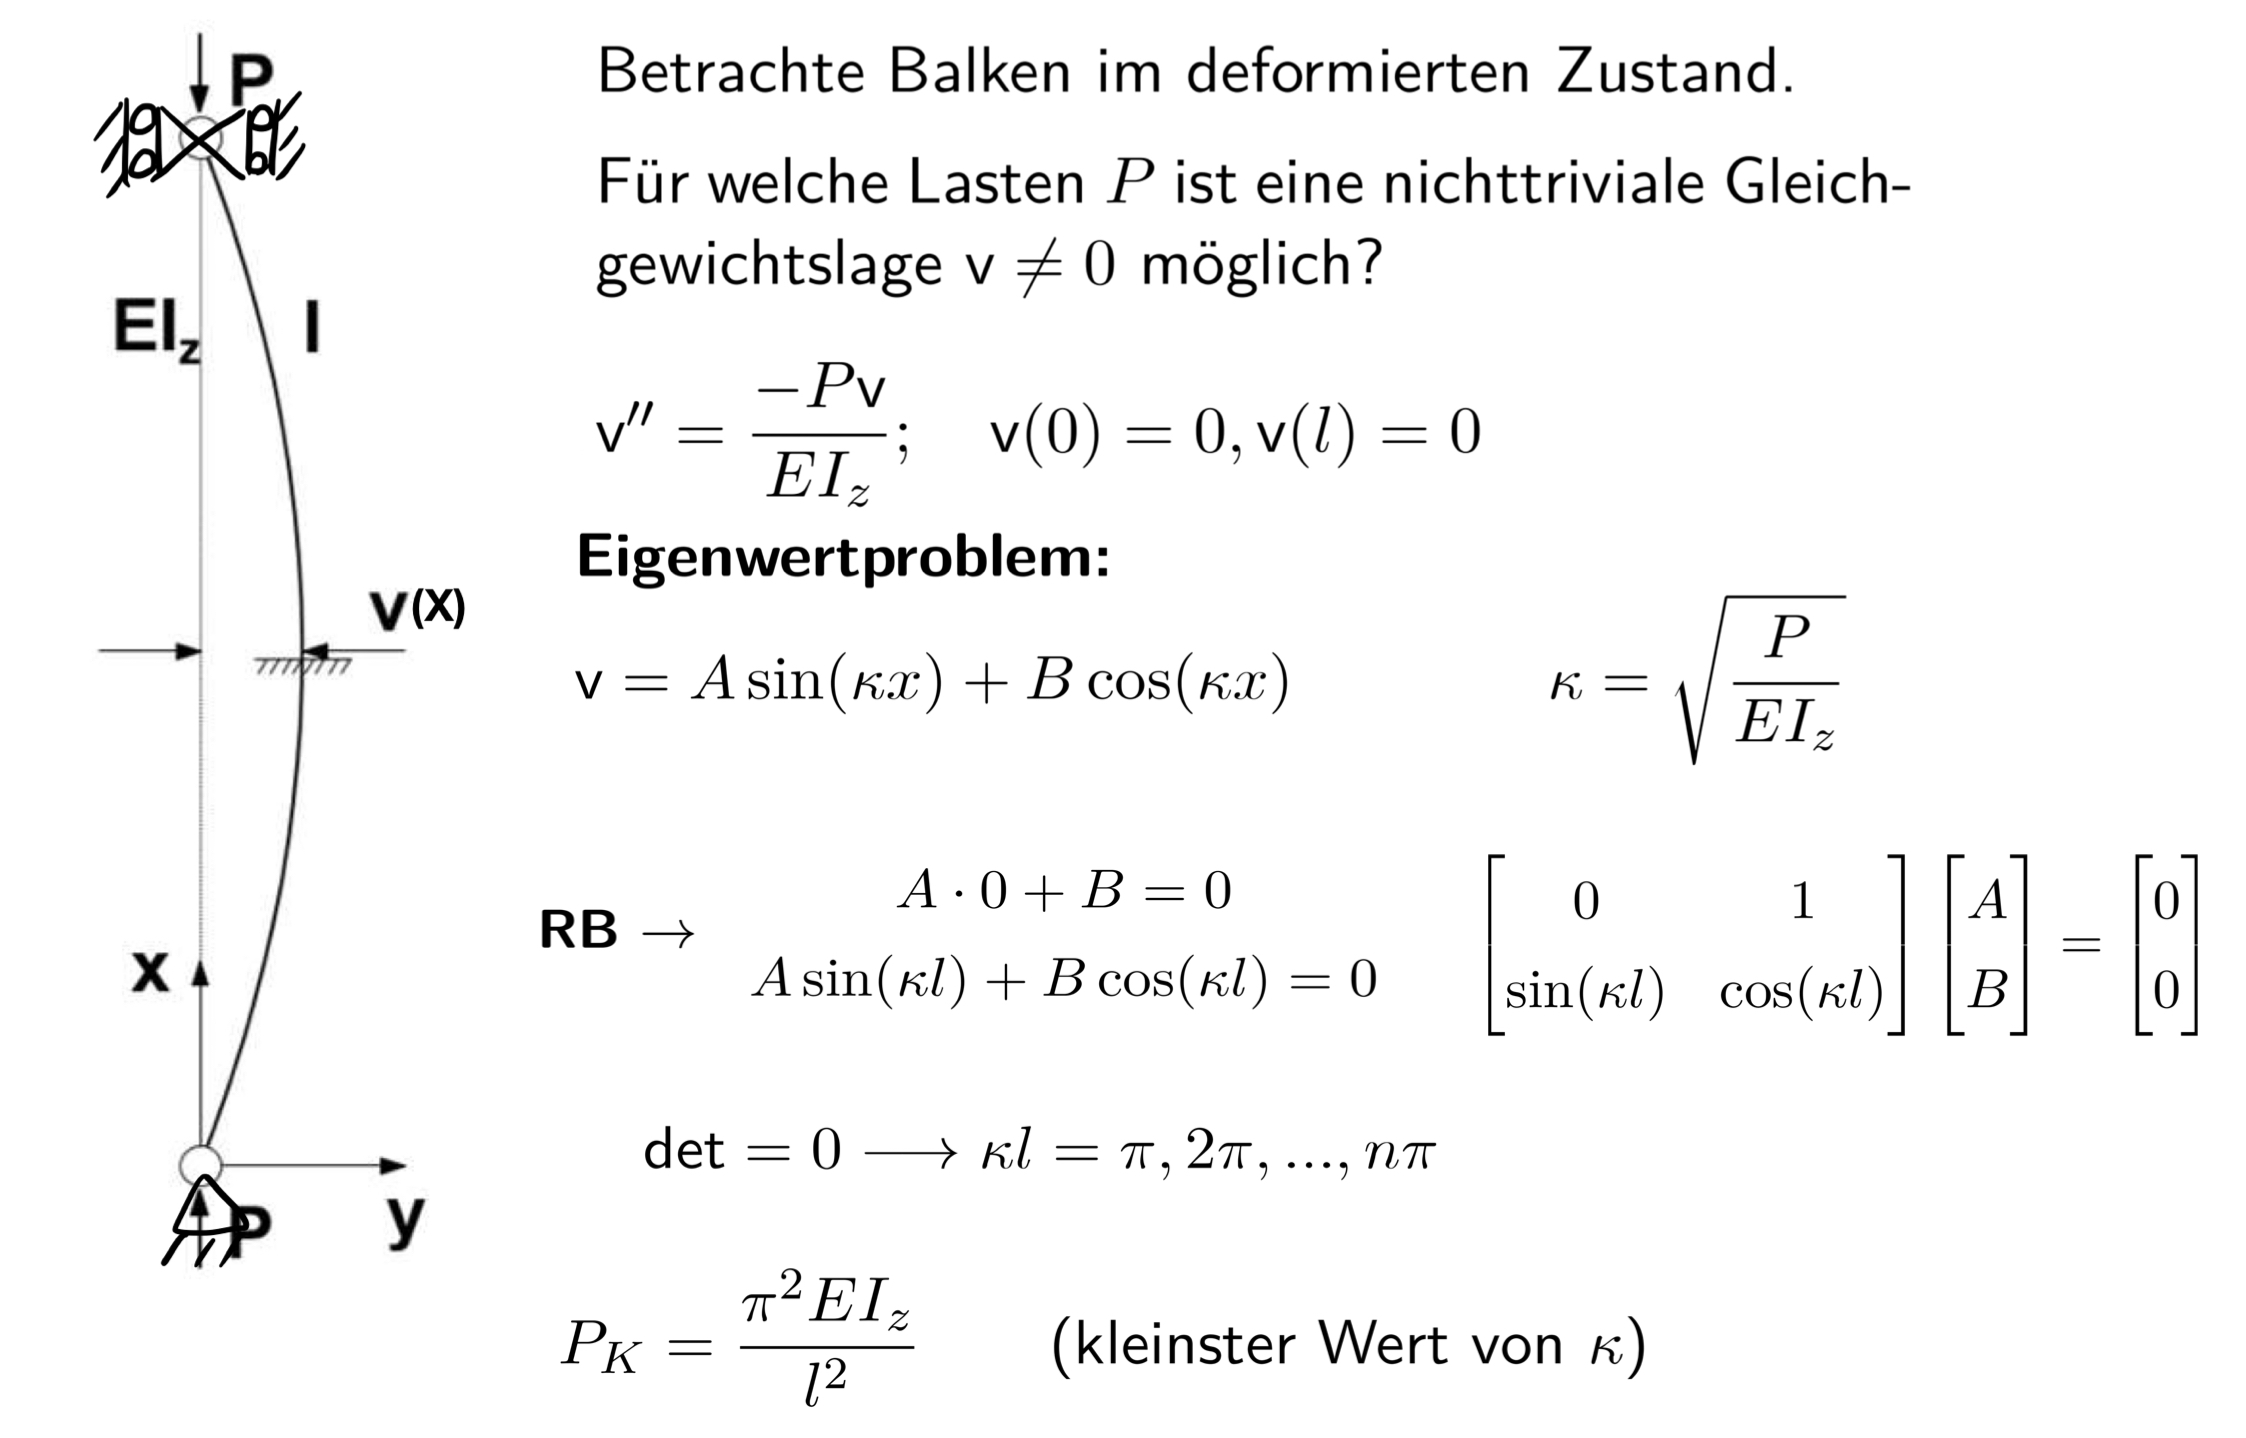
\includegraphics[width=0.9\linewidth]{09/1d.jpeg}
        \end{center}
\columnbreak
        Balken auf einer Seite eingespannt und andere Seite los.
        \begin{center}
            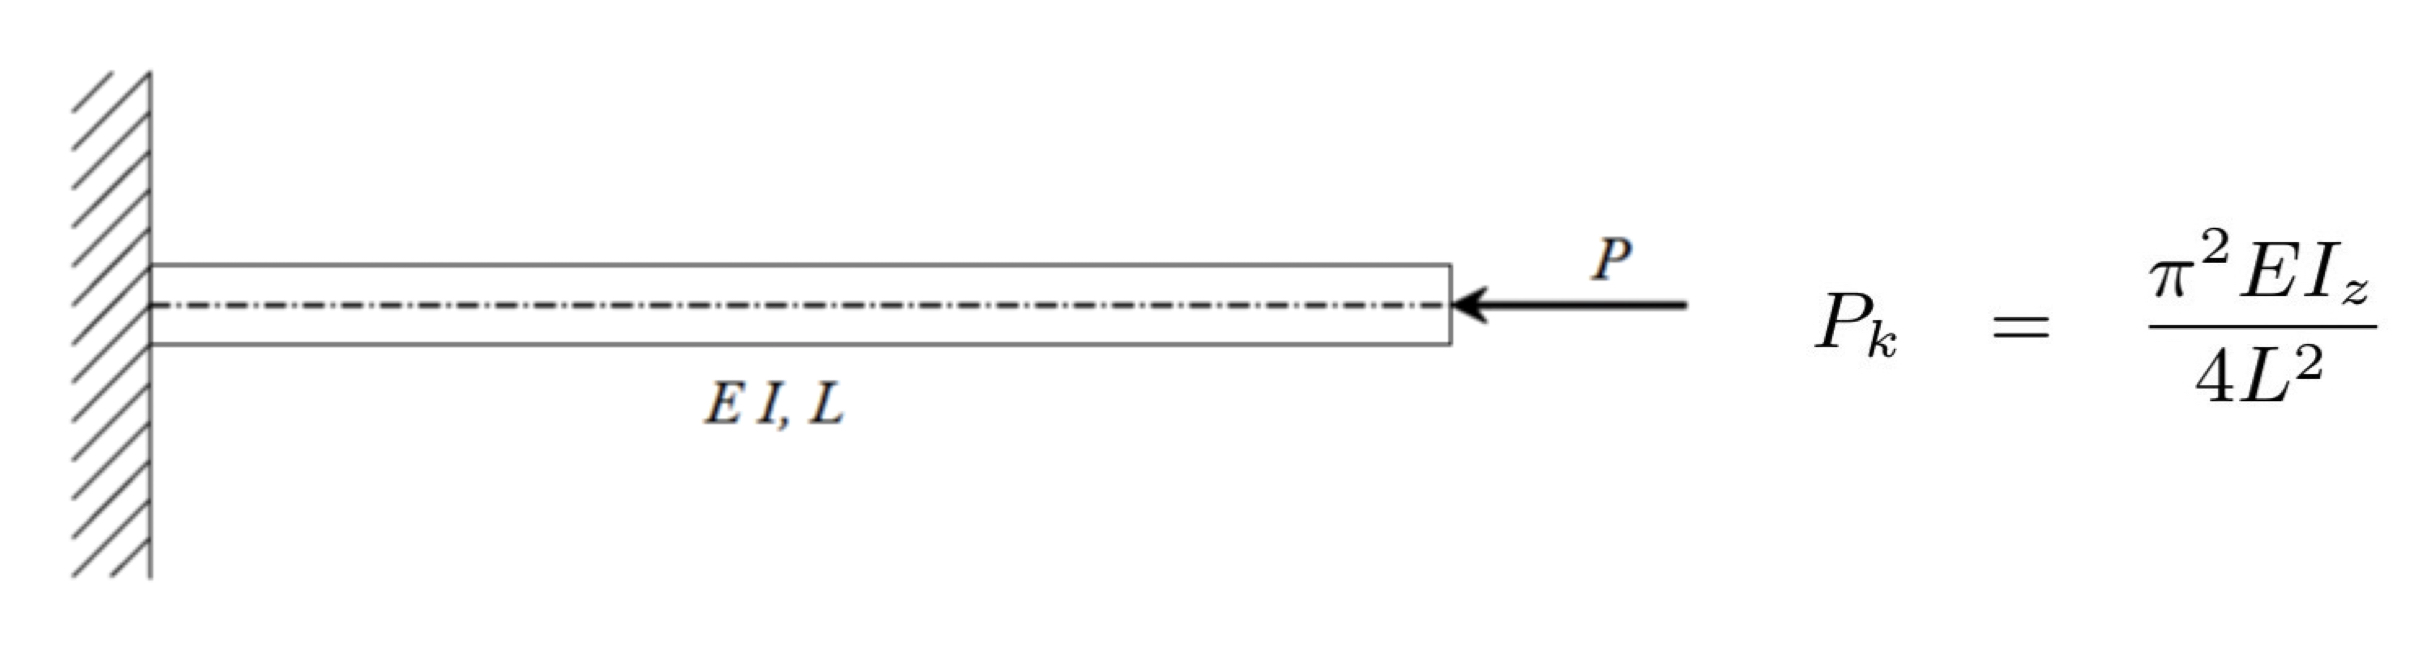
\includegraphics[width=0.8\linewidth]{09/uebung2.jpeg}
        \end{center}
        \begin{center}
             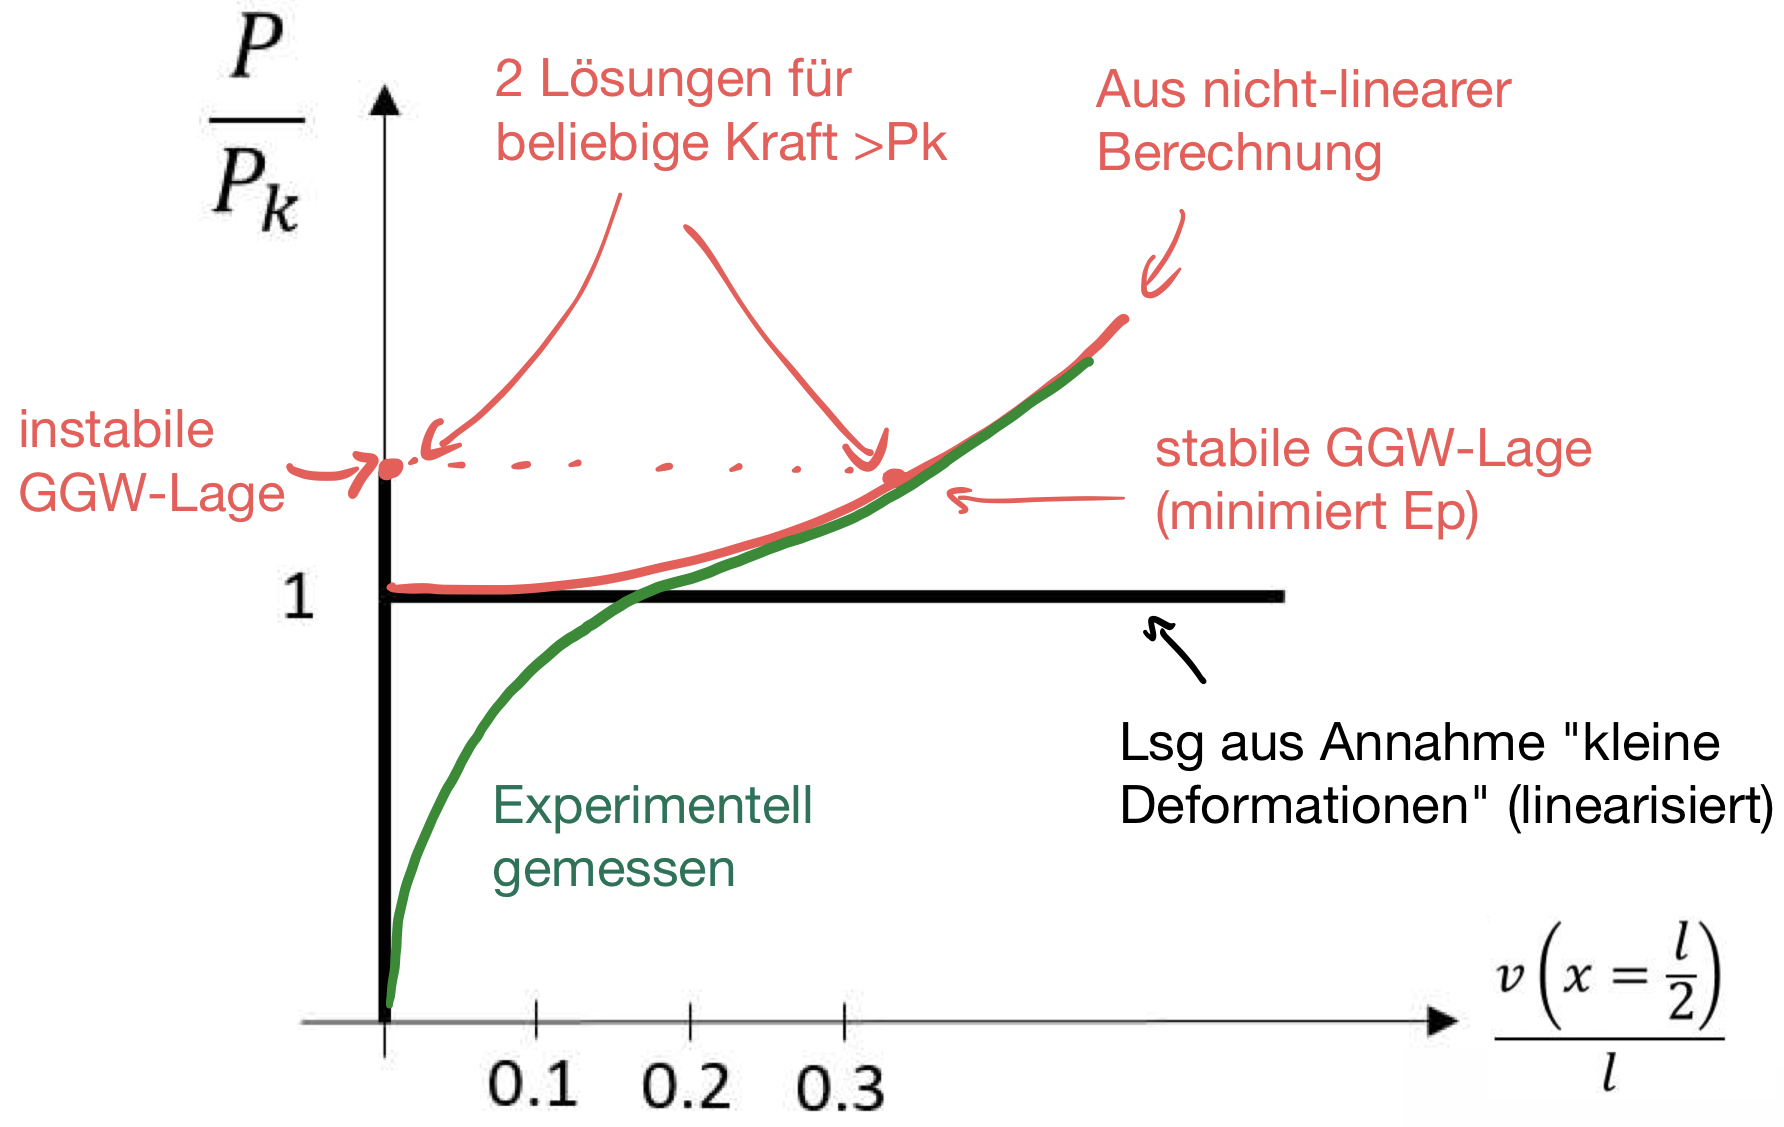
\includegraphics[width=0.8\linewidth]{09/1d-graph2.jpeg}
        \end{center}
        
    \subsection{System mit 1-Freiheitsgrad}
        2 Pendelstützen von Länge $l/2$ gelenkig mit einer Winkelfeder mit Rückstellmoment $M_c=C\cdot\alpha$ verbunden.
        \begin{itemize}
            \item \textbf{linear:} $P=\frac{4C}{l}=P_K$
            \item \textbf{nichtlinear:} $P=P_K\left(1+\frac{2}{3}\left(\frac{q}{l}\right)^2+\frac{6}{5}\left(\frac{q}{l}\right)^4+\dots\right)$ \\mit $P_K=\frac{4C}{l}$
        \end{itemize}
        Bei nichtlinearer Betrachtung mehr als 1 Ruhelage (meist instabil) bei $P\geqslant P_K$ ($q=0$ oder $q >0$) $\rightarrow$ "Verzweigungsproblem"/\textbf{"Bifurkation"}
        \\\textbf{Bei Strukturfehler tritt keine Bifurkation auf!}
        \\\textit{Stabilitätssatz von Lagrange:}\\\\
        In einer Stabilen GGW-Lage hat das Gesamtpotential $E_p$ ein \textbf{Minimum} ($E'_p=0; E''_p>0$)
        \vspace{-2mm}\[E_p = U+V\]
        U: Deformationsenergie (zb. $E_p$ von Feder) 
        \\V: Potential äussere Kräfte
    \subsection{Rayleighscher Quotient}
        \[P_K=\frac{U}{\chi}:=Q\]
        mit $P$: Angriffskraft; \quad $\chi$: Verschiebung der Kraft\\\\
        \textbf{Vorgehen:}
        \begin{enumerate}
            \item Wähle zulässiges Verschiebungsfeld $v(x)$
            \item Finde $\displaystyle U(v) \rightarrow U = \frac{1}{2}EI\int_{0}^{L}(v'')^2dx$ \quad(MechII)
            \item Finde $\displaystyle \chi(v) \rightarrow \chi=\frac{1}{2}\int_{0}^{L}(v')^2dx$ \qquad(Geometrie)
            \item $Q=\frac{U}{\chi}$ Rayleighscher Quotient
            \item $\displaystyle\frac{\partial Q}{\partial\alpha}=0 \textrm{ oder } \frac{\partial Q}{\partial\beta}=0 \rightarrow$ Bedingung für $\alpha \textrm{ und } \beta$
            \item $\Tilde{P}_k=\textrm{min}(Q)$
            
        \end{enumerate}
        